% -*- root: main.tex -*-

\chapter{Loose ends}

\todo[inline]{I'd like to spend a couple of days talking about ways the picture in this class can be extended, finally, some actually unanswered questions that naturally arise.  The following two section titles are totally made up and probably won't last.}
\todo[inline]{Also, write a broad-scale introduction to this appendix.}









\section{The period map}\label{ThePeriodMapSection}

\todo{pp.\ 42-43 of FPFP has some easy-to-state results about this collected.}
\todo{Kohlhaase~\cite{Kohlhaase} references Yu~\cite{Yu} for having closed formulas generalizing the Hopkins--Gross example section.}
\todo{Section 2.3 (pg.\ 35--36) of Morava's \textit{Noetherian Localisations} gives a sketch of the period map (in terms of curves, I guess).}
\todo{Mention that the period map is equivariant for the isotropy action.}

Describe Dieudonn\'e crystals and the Tapis de Cartier.

Show how Dieudonn\'e crystals are used to give formulas for the action of the stabilizer group~\cite{DevinatzHopkins}.

Give a sketch explanation of the Gross--Hopkins period map~\cite{Weinstein}.

Draw the picture of the period map at $n = 2$, $p = 2$.  The main reference for this, except for the literal picture, is~\cite[Appendix 25]{HopkinsGrossEquivVBs}.
\begin{itemize}
\item The center of the $\Z_{p^2}$--points of Lubin--Tate space corresponds to the canonical lift, which is the formal group that further acquires an $\mathcal O_A$--module structure.  It has $\pi$--series $[\pi](x) = \pi x + x^{q^2}$.
\item There are three nontrivial points in $\G[2]$: $\alpha$, $\beta$, and $\alpha + \beta$.  Quotienting by them gives three points at order $1/(q+1)$, the first bunch of ``quasicanonical lifts'', which have partial formal $\mathcal O_A$--module structures.
\item At each quasicanonical point, you also also form three quotients: two of them make the situation ``worse'', and one of them makes the situation ``better''.  This has to do with the identification $\G / \G[2] \cong \G$.
\item Computing these orders has to do with the Newton polygon associated to the $\pi$--series.
\item The canonical Frobenius $F_{can} = \left[ \begin{array}{cc} 0 & p \\ 1 & 0 \end{array} \right]$ first flips the two coordinates (and scales one by $p$), then flips them back (and scales the other by $p$), and after two flips scaling everything by $p$ scales back down by homogeneous coordinates.
\item Out to order $1/q$, $\pi_{GH}$ is injective.
\item The group $\F_4^\times$ should act by rotation on $\mathbb P^1$.
\item The map $\pi_{GH}$ sends the canonical lift to $0 = [1:0]$, sends the first order quasicanonical points to $\infty = [0:1]$, and alternates from there.  The three branches of ``directions to quotient'' carve $\mathbb P^1$ up into three lobes.  This is because $\pi_{GH}$ is equivariant for \emph{isogenies}, and quotienting by one of these order $2$ subgroups is a lift of the Frobenius isogeny on the residue formal group.
\item These quasicanonical points are the ones with nontrivial stabilizers under the action by the Morava stabilizer group---all the other points belong to free orbits.  (The canonical lift has the largest stabilizer of all.)
\end{itemize}

\begin{figure}
\begin{center}

\pgfdeclareradialshading{myshading}{\pgfpointorigin}
{
  color(0cm)=(pgftransparent!100);
  color(2cm)=(pgftransparent!100);
  color(2.5cm)=(pgftransparent!0);
  color(3cm)=(pgftransparent!0)
}
\pgfdeclarefading{fading3}{\pgfuseshading{myshading}}

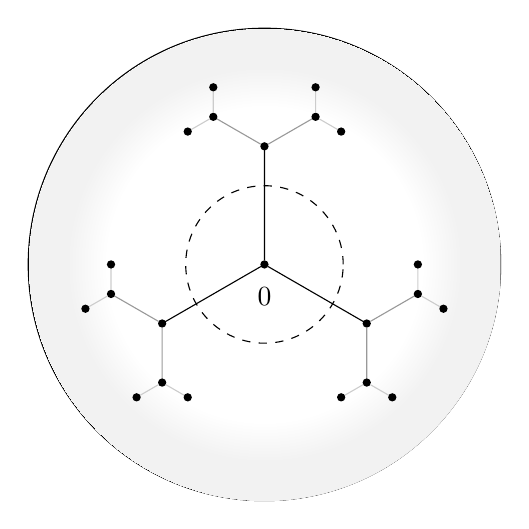
\begin{tikzpicture}[baseline=(current bounding box.center)]
% thanks to Tomasz M. Trzeciak
% based off of http://www.latex-community.org/viewtopic.php?f=4&t=2111

\draw (0,0) circle (3);

\begin{scope}
\pgfsetfading{fading3}{\pgftransformshift{\pgfpoint{0cm}{0cm}}}
\filldraw[black!5] (0,0) circle (3);
\end{scope}

\draw[dashed] (0,0) circle (1);
\coordinate[style={inner sep=0pt, outer sep=0pt, minimum size=3pt, fill=black, circle}] (O) at (0,0);
\node[below=5pt] at (O) {$0$};

\draw (O) -- +( 90:1.5) coordinate[style={inner sep=0pt, outer sep=0pt, minimum size=3pt, fill=black, circle}] (Q1)
      (O) -- +(210:1.5) coordinate[style={inner sep=0pt,outer sep=0pt,minimum size=3pt, fill=black,circle}] (Q2)
      (O) -- +(330:1.5) coordinate[style={inner sep=0pt,outer sep=0pt,minimum size=3pt, fill=black,circle}] (Q3);

\draw[black!40] (Q1) -- +(120-90:0.75) coordinate[style={inner sep=0pt, outer sep=0pt, minimum size=3pt, fill=black, circle}] (Q12)
      (Q1) -- +(240-90:0.75) coordinate[style={inner sep=0pt, outer sep=0pt, minimum size=3pt, fill=black, circle}] (Q13)
      (Q2) -- +(120-330:0.75) coordinate[style={inner sep=0pt, outer sep=0pt, minimum size=3pt, fill=black, circle}] (Q21)
      (Q2) -- +(240-330:0.75) coordinate[style={inner sep=0pt, outer sep=0pt, minimum size=3pt, fill=black, circle}] (Q23)
      (Q3) -- +(120-210:0.75) coordinate[style={inner sep=0pt, outer sep=0pt, minimum size=3pt, fill=black, circle}] (Q31)
      (Q3) -- +(240-210:0.75) coordinate[style={inner sep=0pt, outer sep=0pt, minimum size=3pt, fill=black, circle}] (Q32);

\draw[black!20] (Q12) -- +(90:0.375) coordinate[style={inner sep=0pt, outer sep=0pt, minimum size=3pt, fill=black, circle}] (Q121)
      (Q12) -- +(330:0.375) coordinate[style={inner sep=0pt, outer sep=0pt, minimum size=3pt, fill=black, circle}] (Q123)
      (Q13) -- +(90:0.375) coordinate[style={inner sep=0pt, outer sep=0pt, minimum size=3pt, fill=black, circle}] (Q131)
      (Q13) -- +(210:0.375) coordinate[style={inner sep=0pt, outer sep=0pt, minimum size=3pt, fill=black, circle}] (Q132)
      (Q21) -- +(90:0.375) coordinate[style={inner sep=0pt, outer sep=0pt, minimum size=3pt, fill=black, circle}] (Q212)
      (Q21) -- +(210:0.375) coordinate[style={inner sep=0pt, outer sep=0pt, minimum size=3pt, fill=black, circle}] (Q213)
      (Q23) -- +(210:0.375) coordinate[style={inner sep=0pt, outer sep=0pt, minimum size=3pt, fill=black, circle}] (Q231)
      (Q23) -- +(330:0.375) coordinate[style={inner sep=0pt, outer sep=0pt, minimum size=3pt, fill=black, circle}] (Q232)
      (Q31) -- +(210:0.375) coordinate[style={inner sep=0pt, outer sep=0pt, minimum size=3pt, fill=black, circle}] (Q312)
      (Q31) -- +(330:0.375) coordinate[style={inner sep=0pt, outer sep=0pt, minimum size=3pt, fill=black, circle}] (Q313)
      (Q32) -- +(90:0.375) coordinate[style={inner sep=0pt, outer sep=0pt, minimum size=3pt, fill=black, circle}] (Q321)
      (Q32) -- +(330:0.375) coordinate[style={inner sep=0pt, outer sep=0pt, minimum size=3pt, fill=black, circle}] (Q323);
\end{tikzpicture}%
%
\quad $\xrightarrow{\pi_{GH}}$ \quad%
%
\begin{tikzpicture}[baseline=(current bounding box.center)]

\newcommand\pgfmathsinandcos[3]{%
  \pgfmathsetmacro#1{sin(#3)}%
  \pgfmathsetmacro#2{cos(#3)}%
}
\newcommand\LongitudePlane[3][current plane]{%
  \pgfmathsinandcos\sinEl\cosEl{#2} % elevation
  \pgfmathsinandcos\sint\cost{#3} % azimuth
  \tikzset{#1/.style={cm={\cost,\sint*\sinEl,0,\cosEl,(0,0)}}}
}
\newcommand\DrawLongitudeCircle[2][1]{
  \LongitudePlane{35}{#2} % first argument is angle of elevation
  \tikzset{current plane/.prefix style={scale=#1}}
   % angle of "visibility"
  \pgfmathsetmacro\angVis{atan(sin(#2)*cos(35)/sin(35))} % these are angle of elevation too
  % this might assume that the angle of elevation is positive
  \draw[current plane] (\angVis:1) arc (\angVis:90:1);
  \draw[current plane,dashed] (\angVis:1) arc (\angVis:-90:1);
}

% the "2.5" magic number is the radius of the sphere 
% the "35" magic number is the angle of elevation of the camera
\pgfmathsetmacro\H{2.5*cos(35)}
\filldraw[ball color=white] (0,0) circle (2.5);
\foreach \t in {-5,-125,-245} { \DrawLongitudeCircle[2.5]{\t} }
\coordinate[style={inner sep=0pt,outer sep=0pt,minimum size=3pt,
    fill=black,circle}] (O) at (0,-\H);
\node[below=16pt] at (O) {$0$};
\coordinate[style={inner sep=0pt,outer sep=0pt,minimum size=3pt,
    fill=black,circle}] (I) at (0,\H);
\node[above=16pt] at (I) {$\infty$};
\end{tikzpicture}
\end{center}

\caption{The period map at $n = 2$, $p = 2$}
\end{figure}

\begin{theorem}\citeme{\cite{HopkinsGrossAnnouncement,StricklandGHDuality}}
\todo{Make sure you get this right.}
The sheaf $\context{E_\Gamma}(\mathbb I_{\Q/\Z})$ is the dualizing sheaf on $(\moduli{fg})^\wedge_\Gamma$. \qed
\end{theorem}





\section{Knowns and unknowns}



\subsection*{Higher orientations}

$\TAF$ and friends\label{TAFDiscussion}

The $\alpha_{1/1}$ argument: Prop 2.3.2 of Hovey's $v_n$--elements of ring spectra

% The HLP calculations

\subsection*{Equivariance}

This is tied up with the theory of power operations in a way I've never really thought about.  Seems complicated.

You should also mention the ``rigidity'' of the elliptic genus, which is about an $S^1$--equivariant version.

\subsection*{Index theorems}

Connections with analysis

The Stolz--Teichner program








-----

Bousfield's work on the $K$--theory of infinite loopspaces \cite{BousfieldLambdaRings} and Morava $K$--theoretic analogues of the results of \Cref{LEFTCooperations}
\todo{Ask Mike (and Jacob?) if there are analogues of these results for $kO$ which explain Mahowald's generalized $K$--theoretic Brown--Gitler spectra.  3/29: I did ask Mike, he said he didn't know. I also asked Paul, and he said this seemed unreasonable, since $kO$ isn't valued in co/commutative Hopf algebras.  This is a fair point: one would need to invent an ``analogue'' of Dieudonn\'e theory for $kO$, in the sense that some category it takes values in would have to be identified as abelian, where the category is rigid enough that it often sends fiber sequences to exact sequences in the category.}

Constructing sheaves of spectra on $\moduli{fg}$: the no-go results for $E_\infty$ and $A_\infty$ rings on the flat site.  There's a little MO discussion about it here: \texttt{http://chat.stackexchange.com/transcript/message/35361282\#35361282}.

Contexts for structured ring spectra

Difficulty in computing $\S_d \actson E_d^*$. (Gross--Hopkins and the period map.)

Barry's $p$--adic measures

Fixed point spectra and e.g. $L_{K(2)} \tmf$.

Blueshift, A--M--S, and the relationship to A--F--G?

Does $E_n$ receive an $E_\infty$ orientation?  Does $BP$?  (Johnson--Noel says $BP$ usually does not.  A recent preprint of Lawson says $BP$ is not even $E_\infty$ at $p = 2$!!!)

$p$--divisible groups and transchromatic phenomena

Remark 12.13 of published $H_\infty$ AHS says their obstruction framework agrees with the $E_\infty$ obstruction framework (if you take everything in sight to have $E_\infty$ structures).  This is almost certainly related to the discussion at the end of Matt's thesis about the $MU$--orientation of $E_d$.\todo{Section 12.4 compares doing $H_\infty$ descent with doing $E_\infty$ descent and shows that they're the same (in the case of interest?).}

Hovey's paper on $v_n$--periodic elements in ring spectra.  He has a nice (and thorough!) exposition on why one should be interested in bordism spectra and their splittings: for instance, a careful analysis of $M\Spin$ will inexorably lead one toward studying $KO$.  It would be nice if studying $M\String$ (and potentially higher analogues) would lead one toward non-completed, non-connective versions of $EO_n$.  Talk about $BoP$, for instance.

Matt's short resolutions of chromatically localized $MU$.

Nilpotency and vanishing curves in the ($MU$--)Adams spectral sequence.  The \emph{non}-nilpotency of $\eta$ in the $MU$--Adams spectral sequence.  Mathew--Meier type theorems about horizontal vanishing lines and the Tate construction (and related results about the $\TMF$ spectral sequence and the Johnson--Wilson theories).

Additive degeneration and $kO \ne kU^{hC_2}$.






\begin{remark}
It is completely unclear why $MU$ plays such an important mediating role between geometry (i.e., the stable category) and algebra (i.e., sheaves on the moduli of formal groups).  Given a general ring spectrum $R$ and thick prime $\otimes$--ideals $\CatOf C_\alpha$ of perfect $R$--modules, one ask the analogous two questions:
\begin{enumerate}
\item Is it possible to find an $R$--algebra $S$ whose context functor induces a homeomorphism of Balmer spectra $\Spec(\CatOf{Modules}_R^{\perf}) \to \Spec(\CatOf{QCoh}(\context{S/R}))$?
\item Are there complementary localizers $L_\alpha\co \CatOf{Modules}_R \to \CatOf{Modules}_{R,(\alpha)}$?  Can they be presented via Bousfield's framework as homological localizations for auxiliary $S$--algebra spectra $S_\alpha$?  Do the contexts $\context{S_\alpha}$ admit compatible localizers with $\context{S}$?
\end{enumerate}
For $R = \S$, this is the role that the $R$--algebra $S = MU$ and the $S$--algebras $S_d = E(d)$ play.  Finding these spectra feels like striking gold, and it is unclear how to produce analogous spectra in general.
\todo{Mathews's work on Galois descent shows that the fixed point map $\CatOf{Modules}_{E_\Gamma, \Aut \Gamma}^{\mathrm{complete}} \to \CatOf{Spectra}_{\Gamma}$ is an equivalence of categories.}
\end{remark}
\noindent One can ask the same question from the geometric direction: why bordism?  Why should these spectra have these nice flatness properties?  Why should they have recognizable computational properties?  Why bordism?




\begin{remark}
The homotopy of $\widehat L_2 \S$ is also known, by work of Shimomura and collaborators~\cite{Shimomura,ShimomuraYabeM20,ShimomuraYabeL2S} (but see also the reorganization by Behrens~\cite{BehrensRevisited}).  It is \emph{exceedingly} complicated, and it is an open problem to find an expression of it which admits human digestion.  Behrens has pursued a program encoding this problem in terms of modular forms~\cite{BehrensCongruences,BehrensModularDescription,BehrensBuildings}, and Hopkins has proposed a program involving $L$--functions~\cite{StricklandpAdicInterpolation}, motivated by which Hovey and Strickland have shown a kind of continuity result for among the groups~\cite[Section 14]{HoveyStrickland}.
\end{remark}





\begin{remark}
There are also ``finitary'' flavors of chromatic localization available, which are typically less robust but more computable.  They assemble into a diagram:
\begin{center}
\begin{tikzcd}
E \arrow{r} \arrow{d} & L_d^{\fin} E \arrow{r} \arrow{d} & L_d E \arrow{d} \\
L_{X(d)} E \arrow{r} & \widehat L_d^{\fin} E \arrow{r} & \widehat L_d E,
\end{tikzcd}
\end{center}
where $X(d)$ is a finite complex of type exactly $d$, $v$ is a $v_d$--self-map of $X(d)$, $T(d) = X(d)[v^{-1}]$ is the localizing telescope, $\widehat L_d^{\fin}$ is Bousfield localization with respect to $T(d)$ (which can be shown to be independent of choice of $X(d)$ and of $v$), and $L_d^{\fin}$ denotes localization with respect to the class of \emph{finite} $E(d)$--acyclics.  Many things about these functors are known: for instance, $L_{X(d)} L_d = \widehat L_d$, there is a chromatic fracture square relating $L_d^{\fin}$ to $\widehat L_{\le d}^{\fin}$, and $L_d^{\fin} E \simeq L_d E$ if and only if $\widehat L_{\le d}^{\fin} E \simeq \widehat L_{\le d} E$.  One major question about these functors remains open, corresponding the last unsettled nilpotence and periodicity conjecture of Ravenel~\cite[Conjecture 10.5]{RavenelLocalizationWRTPeriodic}: is the map $\widehat L_d^{\fin} E \to \widehat L_d E$ an equivalence?  Multiple proofs and disproofs have been offered, but the literature remains unsettled.
\citeme{Find some proofs and disproofs.}
\end{remark}







\begin{remark}
Writing $M_d$ for the fiber in the sequence $M_d \to L_d \to L_{d-1}$, the filtration spectral sequence associated to the tower in \Cref{ChromaticConvergence} is called the \textit{geometric chromatic spectral sequence}, which has the form $\pi_* M_* \S \Rightarrow \pi_* \S_{(p)}$.  The two forms of filtration data $M_d X$ and $\widehat L_d X$ are actually functorially equivalent to one another:
\begin{align*}
\widehat L_d M_d & \simeq \widehat L_d, &
M_d \widehat L_d & \simeq M_d,
\end{align*}
but they have fairly distinct properties.  For instance, $M_d$ is smashing whereas $\widehat L_d$ is not, $M_d$ is not part of an adjoint pair whereas $\widehat L_d$ is, and the analogue of \Cref{FormulaForKnLocalization} for $M_d$ is ``backwards'':\citeme{I forget who this is due to} \[M_d X \simeq \colim_I \left( M^0(v^I) \sm L_d X \right).\]  The spectrum $M_d X$ also relates to the chromatic fracture square for $X$:
\begin{center}
\begin{tikzcd}
M_d X \arrow{d} \arrow[equal]{r} & M_d X \arrow{d} \\
L_d X \arrow{r} \arrow{d} \arrow[dr, phantom, "\lrcorner", very near start] & \widehat L_d X \arrow{d} \\
L_{d-1} X \arrow{r} & L_{d-1} \widehat L_d X.
\end{tikzcd}
\end{center}
From this, we see that there is a fiber sequence $M_d X \to \widehat L_d X \to L_{d-1} \widehat L_d X$.

The case $d = 1$ gives the prototypical example of the difference between these two presentations of the ``exact height $d$ data'', where the sequence becomes: \[\colim_j (M^0(p^j) \sm L_1 X) \to \lim_j (M_0(p^j) \sm L_1 X) \to \left( \lim_j (M_0(p^j) \sm L_1 X) \right)_{\Q}.\]  If, for instance, $\pi_0 L_1 X = \Z_{(p)}$, then the long exact sequence of homotopy groups associated to this fiber sequence gives
\begin{center}
\begin{tikzcd}
\pi_0 \widehat L_1 X \arrow{r} \arrow[equal]{d} & \pi_0 L_0 \widehat L_1 X \arrow{r} \arrow[equal]{d} & \pi_{-1} M_1 X \arrow[equal]{d} \\
\Z^\wedge_p \arrow{r} & \Q_p \arrow{r} & \Z/p^\infty.
\end{tikzcd}
\end{center}
Coupling this to \Cref{piLK1SExample}, we compute
\begin{align*}
\pi_t M_1 \S^0 & = \begin{cases} \Z/p^\infty & \text{when $t = -1$}, \\ \Z_p / (pk) & \text{when $t = k|v_1| - 1$ and $t = \ne 0$}, \\ \Z/p^\infty & \text{when $t = (0 \cdot |v_1| - 1) - 1 = -2$}, \\ 0 & \text{otherwise}. \end{cases}
\end{align*}
This is a model for what happens generally when passing from $\pi_* \widehat L_d X$ to $\pi_* M_d X$: the $v_j$--torsion--free groups get converted to infinitely $v_j$--divisible groups, with some dimension shifts.\footnote{A height $2$ example of this same phenomenon is visible in Behrens's paper~\cite[Section 7]{BehrensRevisited}.}
\end{remark}




\begin{theorem}[Unpublished work of Hopkins and Lurie]
Let $F_d$ denote the discrepancy spectrum for $E_d$.  There is a natural equivalence of infinite loopspaces $\Loops^\infty F_d \simeq \Susp^d \mathbb I_{\Q/\Z}$. \qed
\end{theorem}




free $E_\infty$--orientations off of $MU$



At the top fo page 10 Neil talks in FPFP very briefly about Greenlees--May and local homology.






Comparison of comodules $M$ for the isogenies pile with the action of $M_n(\Z_p)$ on $M \otimes_{E_n^*} D_\infty$ (this is a modern result due to Tomer, Tobi, Lukas, and Nat).  This is basically Nat's rational claim: start with a sheaf on the isogenies pile.  Tensor everything with $\Q$.  That turns this thing into a rational algebra under the Drinfel'd ring together with an equivariant action of $\GL_n \Q_p$.





\todo[inline]{Leave a remark in here about this: McClure in BMMS works along similar lines to show that the Quillen idempotent is not $H_\infty$, but he doesn't get any positive results (and, in particular, he can't complete his analysis as we do because he doesn't have access to the $BP$--homology of finite groups and to HKR character theory).  One wonders whether the stuff here does say something about $BP$ as the height tends toward $\infty$.  So far as I know, no one has written much about this.  Surely it remains a bee in Matt's bonnet.}







Sections 5.3-4 of Hopkins's ICM address \textit{Algebraic Topology and Modular Forms} has a discussion of what $\eta$ and $\nu$ have to do with $\tmf$, as well as the construction of some interesting ``topological $\theta$--series'' in the elliptic cohomology of certain Thom complexes.



\todo[inline]{Jacob wrote me an email giving a very slightly fuller sketch of what the DAG perspective on the $\sigma$--orientation is.  Interestingly, it boils down to a fact from projective geometry: there just aren't that many line bundles on projective varieties.  This forces a couple of things to become equal, and in a suitable setting they even become canonically equal.  The email has no subject line, which will make it hard to find, but you should include a summary of it (which is dependent on whatever's written in the \textit{Survey} paper) all the same.}



